\section{The Problem}
 \begin{wrapfigure}{r}{0.30\columnwidth}
\vspace{-3em}
		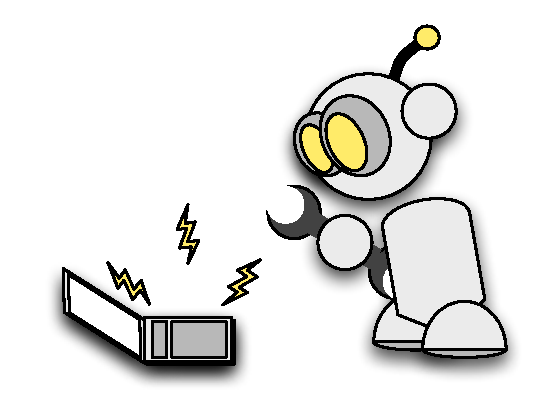
\includegraphics[width=0.30\columnwidth]{diagrams/robot_mechanic.pdf}
 \end{wrapfigure}

Pathfinding in modern video games often involves exploring highly regular 
environments such as cities, sewers or dungeons -- see for example
Figure \ref{fig:iw2}.
These locations are usually highly symmetric in the sense that many optimal 
length paths exist between arbitrary pairs of locations.
Symmetry is undesirable as it increases the size of the search space and forces
search algorithms to waste time.
\newline \newline
In this work we \textbf{speed up pathfinding} by identifying and eliminating
symmetry \textbf{in 4-connected grid maps}.
Our method is fast, optimal, memory efficient and readily combined with any
existing pathfinding system.

 \begin{figure}[h]
	\vspace{1em}
	\centering
	\label{fig:iw2}
		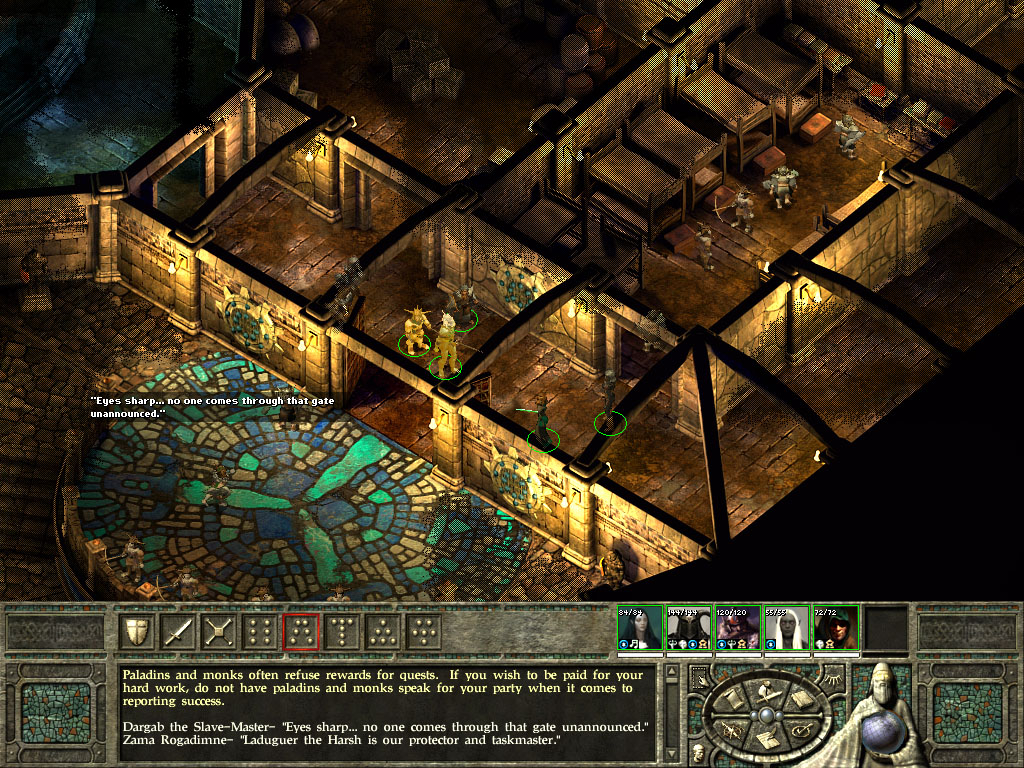
\includegraphics[width=\columnwidth]{diagrams/iwdale.jpg}
 \caption{A dungeon from BioWare's Icewind Dale II}
 \end{figure}

